\documentclass{article}
\usepackage{spconf,amsmath,graphicx}
\usepackage{amssymb}
\usepackage{enumitem}
\usepackage{hyperref}

\title{Optimizing DTW-Based Audio-to-MIDI Alignment and Matching}

\name{Colin Raffel and Daniel P. W. Ellis}
\address{LabROSA\\
    Columbia University\\
    New York, NY}

\begin{document}
\ninept
\maketitle

\begin{abstract}
Dynamic time warping (DTW) has proven to be an extremely effective method for both aligning and matching recordings of music to corresponding MIDI transcriptions.
However, its performance is heavily affected by factors such as the representation used for the audio and MIDI data and its adjustable parameters.
We therefore investigate automatically optimizing the design of DTW-based alignment and matching systems.
Our approach uses Bayesian optimization to tune system design and parameters over a synthetically-created dataset of audio and MIDI pairs.
We then perform an exhaustive search over DTW score normalization techniques to find the optimal method for reporting a reliable alignment confidence score, as required in matching tasks.
This results in a DTW-based system which is conceptually simple and highly accurate at both alignment and matching.
We verified that this system achieves high performance in a large-scale qualitative evaluation of real-world alignments.
\end{abstract}

\begin{keywords}
Dynamic Time Warping, Audio to MIDI Alignment, Sequence Retrieval, Bayesian Optimization, Hyperparameter Optimization
\end{keywords}

\section{Introduction}
\label{sec:intro}

Widely-available MIDI versions of popular music tracks can provide a bounty of ground-truth data for content-based music information retrieval tasks, including beat/bar tracking, onset detection, key estimation, automatic transcription, and score-informed source separation (see e.g.\ \cite{ewert2012towards, turetsky2003ground, ewert2014score, raffel2014pretty_midi}).
However, to maximize its value, a given MIDI file must be aligned in time to a corresponding music audio file.
This alignment problem is closely related to MIDI-to-audio matching, which seeks to identify which  audio file (if any) corresponds to a given MIDI in independent MIDI and audio file collections.
This problem is motivated by the dearth of metadata information typically available in MIDI files, making any kind of text-based matching infeasible \cite{raffel2015large}.
In both scenarios, it is of great value to produce an alignment confidence score which communicates how well the content in a MIDI file matches a given audio file, which can reflect the transcription quality.

Most previous research has focused on systems meant for either alignment or matching but not both.
In the context of MIDI-to-audio alignment, a wide variety of techniques have been proposed to determine a correspondence between discrete times in the audio and MIDI files.
While some approaches use edit distance measures such as Smith-Waterman \cite{ewert2012towards} and Needleman-Wunsch \cite{grachten2013automatic}, the most common approach is dynamic time warping (DTW) \cite{muller2007dynamic}.
First proposed for comparing speech utterances \cite{sakoe1978dynamic}, DTW uses dynamic programming to find a monotonic alignment such that the sum of a distance-like cost between aligned feature vectors is minimized.
This property makes it well-suited for audio-to-MIDI alignment when we expect that the MIDI is an accurate continuous transcription (i.e.\ without out-of-sequence or incorrect sections).

Since the total distance between aligned pairs of feature vectors gives a single global value, one nice outcome of DTW is a natural measure of the ``similarity'' between two sequences.
In fact, DTW has seen extensive use as a way of measuring sequence similarity in the data mining literature \cite{berndt1994using}.
In the context of MIDI and audio files, \cite{hu2003polyphonic} evaluated DTW's effectiveness at matching a small collection of Beatles MIDIs to recordings of Beatles songs.

Despite its widespread use, DTW's success is dependent on its parametrization as well as system design choices such as the feature representation and the local distance metric used.
To our knowledge, there has been no large-scale quantitative comparison of different DTW-based alignment systems.
This is likely due to the fact that evaluating a given system's performance would require either a large collection of MIDI and audio pairs for which the correct alignment is already known (which does not exist) or manual audition and rating of the output of the systems (which is time-consuming).

The present work aims to remedy this by searching across a large space of DTW designs to optimize both alignment accuracy and confidence reporting.
After giving an overview of typical DTW-based alignment systems (Section \ref{sec:dtw}), we propose a method for creating a synthetic dataset of MIDI-audio pairs by applying realistic corruptions to MIDI files, allowing us to know a priori the correct alignment (Section \ref{sec:synthetic}).
We then tune parameters for alignment using Bayesian optimization (Section \ref{sec:optimizing}) and for confidence reporting using an exhaustive search (Section \ref{sec:confidence}).
Finally, we perform a large-scale qualitative evaluation of our proposed alignment system on real-world data and discuss possibilities for improvement (Section \ref{sec:qualitative}).

\section{DTW-Based Alignment}
\label{sec:dtw}

Suppose we are given two sequences of feature vectors $X \in \mathbb{R}^{M \times D}$ and $Y \in \mathbb{R}^{N \times D}$, where $D$ is the feature dimensionality and $M$ and $N$ are the number of feature vectors in $X$ and $Y$ respectively.
Dynamic time warping produces two nondecreasing sequences $p, q \in \mathbb{N}^L$ which define the optimal alignment between $X$ and $Y$, such that $p[i] = n, q[i] = m$ implies that the $m$th feature vector in $X$ should be aligned to the $n$th in $Y$.
In DTW, finding $p$ and $q$ involves solving the following minimization problem:
$$
p, q = \mathrm{arg}\min_{p, q} \sum_{i = 1}^{L} \|X[p[i]] - Y[q[i]]\|_2^2 + \Phi(i)
$$
where $\Phi(i)$ is $\phi \ge 0$ when $p[i] = p[i - 1]$ or $q[i] = q[i - 1]$ and $0$ otherwise.
$\phi$ is a constant which is used to discourage ``non-diagonal moves'', i.e.\ indices in the path where a feature vector in one sequence is mapped to multiple vectors in the other.
This minimization problem can be solved in $\mathcal{O}(MN)$ time using dynamic programming \cite{sakoe1978dynamic}.
Once $p$ and $q$ are found, the original MIDI file can be adjusted so that events which occur at $t_X[p[i]]$ are moved to $t_Y[q[i]]$, where $t_X \in \mathbb{R}^M, t_Y \in \mathbb{R}^N$ are the times corresponding to the feature vectors in $X$ and $Y$ respectively.

DTW is often constrained so that $p$ and $q$ span the entirety of $X$ and $Y$, i.e.\ $p[1] = q[1] = 1$ and $p[L] = N; q[L] = M$.
However, audio-to-MIDI alignment systems typically allow subsequence matching (to handle, for example, the case of a MIDI file that covers only a portion of a song), where instead we only require that either $gN \le p[L] \le N$ or $gM \le q[L] \le M$.
$g \in [0, 1]$ (the ``gully'') is a parameter which determines the proportion of the subsequence which must be successfully matched.
In addition, the path is occasionally further constrained so that
$$
q[i] - p[i] + R \le N, p[i] - q[i] + R \le M
$$
for $i \in \{1, \ldots, L\}$ where $R = g\min(M, N)$ is the ``radius'', sometimes called the Sakoe-Chiba band \cite{sakoe1978dynamic}.
A further constraint on $p$ and $q$ is monotonicity; audio to MIDI alignment systems typically enforce this by requiring $p[i + 1] = p[i] + 1$ and/or $q[i + 1] = q[i] + 1$, although other ``step patterns'' have been proposed \cite{muller2007dynamic, sakoe1978dynamic}.

Design choices differentiating DTW systems include:
\begin{description}[topsep=1pt,itemsep=-1pt,leftmargin=5pt]
\item[Feature representation ($X$ and $Y$):] Prior to alignment, audio and MIDI data must be converted to an intermediate representation where their distance can be computed.
This is often done by synthesizing the MIDI file to obtain an audio signal and computing a common spectral transform of the audio recording and synthesized MIDI audio.
Chroma vectors, which represent the amount of energy in each semitone summed across octaves \cite{fujishima1999realtime} are a common choice \cite{hu2003polyphonic, ewert2012towards}.
A constant-Q transform (CQT), which represents the amount of energy in logarithmically spaced bins \cite{brown1991calculation} has also been used \cite{raffel2015large, dixon2005match, ellis2013aligning}.
Occasionally, log-magnitude features are used in order to more closely mimic human perception \cite{raffel2015large, ellis2013aligning, turetsky2003ground}.
In \cite{turetsky2003ground} and \cite{hu2003polyphonic} it is noted that Mel-Frequency Cepstral Coefficients result in poor performance for music signals because they obscure pitch information.
\item[Time scale ($t_X$ and $t_Y$):] Feature vectors are frequently computed over short, overlapping frames of audio \cite{dixon2005match, turetsky2003ground, hu2003polyphonic}.
Note that the spacing between feature vectors must be sufficiently small compared to the auditory temporal resolution, e.g.\ tens of milliseconds \cite{blauert1997spatial}.
Occasionally, beat-synchronous feature vectors are used \cite{raffel2015large,ellis2013aligning}, which can reduce computation time and can produce accurate alignments provided that the beat tracking is correct.
\item[Normalization:] In \cite{rakthanmanon2012searching}, it is argued that z-scoring (standardizing) the feature sequences is critical for data mining applications of DTW, which was used in audio-to-MIDI alignment in \cite{hu2003polyphonic}.
In addition, various normalizations have been applied to the feature vectors in $X$ and $Y$ before computing their local distances.
A common choice is normalizing each vector by its $L^2$ norm, which is equivalent to using the cosine distance \cite{turetsky2003ground, ewert2012towards, raffel2015large, ellis2013aligning}.
\item[Penalty ($\phi$):] In many applications of DTW to audio-to-MIDI alignment, no additive penalty is used, which corresponds to setting $\phi = 0$.
However, as long as the MIDI and audio files have consistent tempi, non-diagonal moves should be discouraged.
In addition, it has been argued \cite{raffel2015large} that when subsequence alignment is allowed, an additive penalty can be crucial to ensure that the entire subsequence is used, and so $\phi$ is set to the 90th percentile of the distances $\|X[n] - Y[m]\|_2^2$ for $m \in \{1, \ldots, M\}; n \in \{1, \ldots, N\}$.
In \cite{ellis2013aligning}, a fixed value of $\phi = .5$ is used.
\item[Gully ($g$) and band path constraint:] The ``gully'' and band path constraint are also often omitted, which corresponds to setting $g = 1$.
A value of $g$ which is close to 1 will afford some tolerance to the possibility that the beginning or end of the MIDI transcription is incorrect (e.g.\ a fade-out or lead-in), so \cite{ellis2013aligning} sets $g = .7$ and \cite{raffel2015large} sets $g = .95$.
In data mining applications \cite{ratanamahatana2004everything} it is argued that the band radius path constraint both reduces computational complexity and results in more reliable alignments by avoiding paths with many non-diagonal moves.
\end{description}

\section{Creating a Synthetic Alignment Dataset}
\label{sec:synthetic}

The list above defines a large space of parameter settings/design choices for DTW-based audio-to-MIDI alignment systems.
Previous research has typically involved manually tuning alignment parameters based on a modest-sized test set of MIDI/audio pairs and informally auditioning the aligned MIDI data.
Because this method only facilitates small-scale comparisons, there is an obvious question of what parameter settings would yield the best general-purpose alignment system.
Unfortunately, manual audition of even a tiny subset of possible parameter settings on a modestly-sized collection of paired MIDI and audio files is infeasible, let alone a collection large enough to make substantive judgements about the general performance of a given system.
Furthermore, automatic evaluation has been blocked by the lack of a large ground-truth dataset of ``correct'' alignments.
We therefore propose a method for synthetically creating MIDI/audio pairs with known alignments by applying a series of corruptions to MIDI files to resemble real-world conditions.
When applying the corruptions, we keep track of the adjustments needed to correctly align the corrupted MIDIs, which allows us to rapidly and automatically evaluate a huge number of possible systems.

To create this dataset, we first collected 1,000 MIDI files which were transcriptions of Western popular music songs.
We then applied the following series of transformations, based on our experience with common differences between MIDI transcriptions and audio recordings:
First, to simulate differences in tempo, we adjusted the timing in each MIDI file by a low-frequency length-$N$ random signal $r$, defined as
\begin{align*}
s[k] &\sim \mathcal{N}(0, \sigma_t), k \in \{0, \ldots, N\}\\
R[k] &= \begin{cases}
s[k]e^{-k}, &k \in \{0, \ldots, N\}\\
R[2N - k], &k \in \{N + 1, \ldots, 2N - 1\}
\end{cases}\\
r[n] &= \sum_{k = 0}^{2N - 1} R[k]e^{j\pi kn/N}, n \in \{0, N - 1\}
\end{align*}
i.e.\ the inverse discrete Fourier transform of an exponentially decaying Gaussian-distributed random spectrum with standard deviation $\sigma_r$.
Second, the first 10\% and last 10\% of the transcription were each cropped out with probability 50\%, which simulates the MIDI file being an incomplete transcription.
In addition, 1\% of each transcription was cut out at a random location with 10\% probability, which simulates a missing measure.
Third, because it is common for a MIDI transcription to be missing an instrument (for example, karaoke versions of songs, in which the lead vocal line has been deleted, are frequently distributed as MIDI files), we removed each instrument track in each MIDI file with probability $p_r$, making sure never to remove all instruments.
Fourth, in all MIDI files, we randomly added 1 or -1 to the program number of each instrument.
This simulated the fact that when comparing a synthesized MIDI file to an audio recording, the timbre of a synthesized MIDI instrument is always somewhat different from its real-world counterpart.
Finally, for each note in each instrument, we multiplied the velocity by a random number sampled from $\mathcal{N}(1, \sigma_v)$ while keeping it in the MIDI velocity range $[1, 127]$.
This was meant to further simulate differences in instrument characteristics in real-world vs.\ synthesized songs, and also simulated missing notes for large $\sigma_v$.
All MIDI data manipulations were realized with \texttt{pretty\char`_midi} \cite{raffel2014pretty_midi}.

As described in Section \ref{sec:intro}, a DTW-based alignment system can serve two purposes: First, to align a MIDI transcription in time to an audio recording, and second, to produce a confidence score denoting the quality of the transcription or whether the MIDI file is a transcription of the recording at all.
We therefore produced two sets of corrupted versions of the 1,000 MIDI files we collected, one to measure alignment performance, and one to evaluate confidence reporting.
For the first (``easy'') set, we focused on corruption parameters corresponding to real-world conditions for a high-quality transcription, setting $\sigma_t = 5, p_r = .1, \sigma_v = .2$.
For the second (``hard''), we set $\sigma_t = 20, p_r = .5, \sigma_v = 1$ so that the alignment task is sufficiently difficult to result in a significant number of incorrect alignments, which allows us to test whether an alignment system can automatically report failure.

\section{Optimizing DTW-Based Alignment}
\label{sec:optimizing}

Given a dataset of MIDI/audio pairs with known correct alignments, we can evaluate a given alignment scheme via the mean absolute alignment error across the set.
The mean error quantifies the extent to which the alignment was able to remove the timing distortions (random warping and cropping) described in Section \ref{sec:synthetic}.
When the alignment has failed for a portion of the song, the error between the mapped times and the correct times may be very large, so we clip the mean error to $.5$ seconds (which essentially denotes an error threshold above which all local alignment discrepancies are equally incorrect).  Thus, our error metric is:
$$
\frac{1}{L}\sum_{i = 1}^{L} \min(|t_X[p[i]] - \hat{t}_X[q[i]]|, 0.5)
$$
where $\hat{t}_X$ is the ground-truth ``warped'' time scale.  We average this measure across the test set.

Rapid calculation of this precise metric (over the ``easy'' test set) allows us to perform large-scale comparisons of different parameter settings.
To decide which settings to try, we use Bayesian optimization, which approximates the relationship between parameter settings and objective values as a Gaussian process.
Using this formulation, Bayesian optimization can automatically propose new alignment systems based on the performance of previously-evaluated systems.
A more thorough discussion can be found in \cite{snoek2012practical}, which is the framework used in this experiment.

Based on the design choices outlined in Section \ref{sec:dtw}, we chose to optimize over the following parameter space:
\begin{description}[topsep=1pt,itemsep=-1pt,leftmargin=5pt]
\item[Feature representation:] We used either chroma vectors or constant-Q spectra.
The constant-Q spectra spanned 4 octaves, starting from MIDI note C3 (65.4 Hz) with 12 bins per octave.
In preliminary experiments, we found that all of the best-performing alignment systems used log-magnitude features regardless of whether chroma vectors or constant-Q spectra were used, so we computed log-magnitude features in all experiments.
\item[Time scale:] We either computed feature vectors every 46 milliseconds or utilized beat-synchronous features.
\item[Normalization:] We optionally z-scored the feature vectors, and normalized them by their $L^1$, $L^2$, $L^\infty$ (max) norm, or not at all.
\item[Penalty:] For the penalty, we optimized a scale in $[0, 3]$ to apply to the median distance between all pairs of feature vectors in $X$ and $Y$.
Using the median distance made this penalty adaptive to different feature representations and normalization schemes.
\item[Gully and band path constraint:] We allowed the gully to take any value in $[0, 1]$ and optionally enforced the band path constraint.
\end{description}
This space subsumes most of the systems discussed in Section \ref{sec:dtw}.
All feature extraction was realized with \texttt{librosa} \cite{mcfee2015librosa, mcfee2015librosa_scipy}.

When performing Bayesian optimization, it is helpful to ``seed'' the optimization with objective values for many randomly-chosen parameter settings to ensure that the optimization thoroughly explores the possible parameter space.
We computed the accuracy for 10,000 randomly configured alignment systems and seeded the optimizer with the 100 systems which achieved the lowest mean error.
In order to avoid local minima in the parameter space, we carried out 10 differently initialized Bayesian optimization runs with 100 trials each, resulting in 1,000 total trials.

The best-performing alignment system achieved an objective value of $0.0181$, meaning that the average absolute error across the entire dataset was about 18 milliseconds.
This is both close to the limit of the auditory temporal resolution and less than half of the time-scale resolution used for non-beat-synchronous feature vectors, so attaining a higher accuracy is likely unrealistic.
A one-sample $t$-test was performed to determine which systems gave alignment quality statistically equivalent to the best performance. Testing the per-pair scores rather than the mean error across all pairs gave better robustness to outliers.  Using a $p$-value of $0.05$ as the threshold returned 51 configurations of indistinguishable quality.

As a high-level overview of these systems, none used beat-synchronization or a path constraint and all of them used log-magnitude constant-Q spectra as a feature representation and set both the penalty median scale and ``gully'' close to 1.
Almost all of these systems used $L^2$ normalization (resulting in a cosine distance for local feature comparisons); a few used $L^1$ normalization.
There was no clear trend in the use of z-scoring.

\section{Optimizing Confidence Reporting}
\label{sec:confidence}

Having found alignment systems which achieve high accuracy on the ``easy'' dataset, we move on to  the question of computing reliable alignment confidence scores.
As described in Section \ref{sec:dtw}, DTW provides a ``raw'' distance as the sum of distances between all aligned feature vectors, such that a small distance denotes high confidence.
This measure is inappropriate, however, when the number of aligned feature vectors varies from song to song; in this setting, the mean distance is usually used instead of the total distance.
Furthermore, it's not  clear if the non-diagonal path penalties $\phi$ should be included in this distance.
Finally, \cite{raffel2015large} advocates further normalizing this distance by
$$
\frac{1}{L^2} \sum_{i = \min(p)}^{\max(p)} \sum_{j = \min(q)}^{\max(q)} \|X[i] - Y[j]\|_2^2
$$
i.e.\ the mean distance between all pairs of frames over the entire aligned portion of both feature sequences.

To choose an optimal confidence measure, we first aligned all of the MIDI/audio pairs in both the ``hard'' and ``easy'' datasets.
Then, for every alignment system generated during our Bayesian optimization trials, we computed the confidence score for every MIDI/audio pair using all combinations of the normalization schemes listed above (with and without length normalization, diagonal penalties, and mean distance normalization) resulting in 8 possible confidence scores per file pair.
Finally, we computed the Kendall rank correlation coefficient \cite{kendall1938new} between each confidence score and the mean absolute error produced by all alignment systems for every pair in both datasets.
A high correlation indicates that the system is able to accurately report the quality of its alignments.

Among our 51 highest-accuracy systems, the highest correlation was 0.710.
In general, the high-accuracy systems all produced rank correlations close to this value.
All of the systems achieved the highest correlation when including the penalties in the score calculation, normalizing by the path length, and normalizing by the mean distance across the aligned portions.
This suggests that these steps are helpful for producing a reliable confidence score.

As a final step in producing a ``gold standard'' alignment system, we decided to find parameter settings that were easy to report and implement but nevertheless produced alignments and confidence scores which were not significantly different than the best systems.
We chose the following design: For a feature representation, we used log-magnitude constant-Q transforms computed on the non-beat-synchronous time scale described in Section \ref{sec:optimizing}.
We normalized the spectra by their $L^2$ norm and did not z-score them.
We chose a penalty $\phi$ as the median distance of all pairs of frames and used a gully parameter $g$ of $0.96$.
This system achieved a mean absolute alignment error on the ``easy'' dataset of 0.0188, with alignment errors which were not significantly different from the best-performing system.
By normalizing the DTW distance (including penalties) by the path length and the mean distance across aligned portions, we achieved a rank correlation between confidence and accuracy of 0.700.
This ``gold standard'' system is straightforward to implement, and will be used for the remainder of this work.

\section{Qualitative Evaluation on Real-World Data}
\label{sec:qualitative}

In the experiments described above, we have found a system which can provide both high accuracy and a useful confidence measure on synthetic data.
To determine its applicability outside of synthetic contexts, we performed a large-scale qualitative evaluation on real-world data.
The dataset used was a randomly chosen set of 500 MIDI/audio pairs from the 25,000-pair ``clean MIDI dataset'' \cite{raffel2015large}, obtained by matching MIDI files with reliable metadata to entries in the Million Song Dataset \cite{bertin2011million} via a fuzzy text match.
This collection comprises MIDI files with a full range of transcription qualities, and includes some pairs which are incorrectly matched due to failure of the text matching procedure.
By manually evaluating whether each resulting alignment was successful, we can determine how accurately the ``gold standard'' system performs alignments and how reliable the reported confidence scores are.

After aligning all pairs in this dataset, we synthesized the resulting aligned MIDI files and created stereo recordings with the aligned synthesized MIDI audio in one channel and the original audio recording in the other.
We then listened to each aligned MIDI pair and annotated a score from 1-5 as follows:
\begin{enumerate}[topsep=1pt,itemsep=-1pt]
\item MIDI and audio file are incorrectly matched
\item Alignment failed due to major differences
\item Alignment was mostly successful with minor issues
\item Perfect alignment with minor transcription issues
\item Perfect alignment and transcription
\end{enumerate}
For example, if a MIDI transcription was matched and successfully aligned to the correct song but was missing an instrument, a rating of 4 would be given; if the missing instrument caused the alignment to sound ``sloppy'', the rating would be 3 instead.
Ideally, alignments with low confidence scores (normalized DTW distance) will be given higher ratings, and vice versa.
To prevent biasing the results, we did not have access to the reported confidence score while rating a given aligned pair.

\begin{figure}[t]
  \centering
  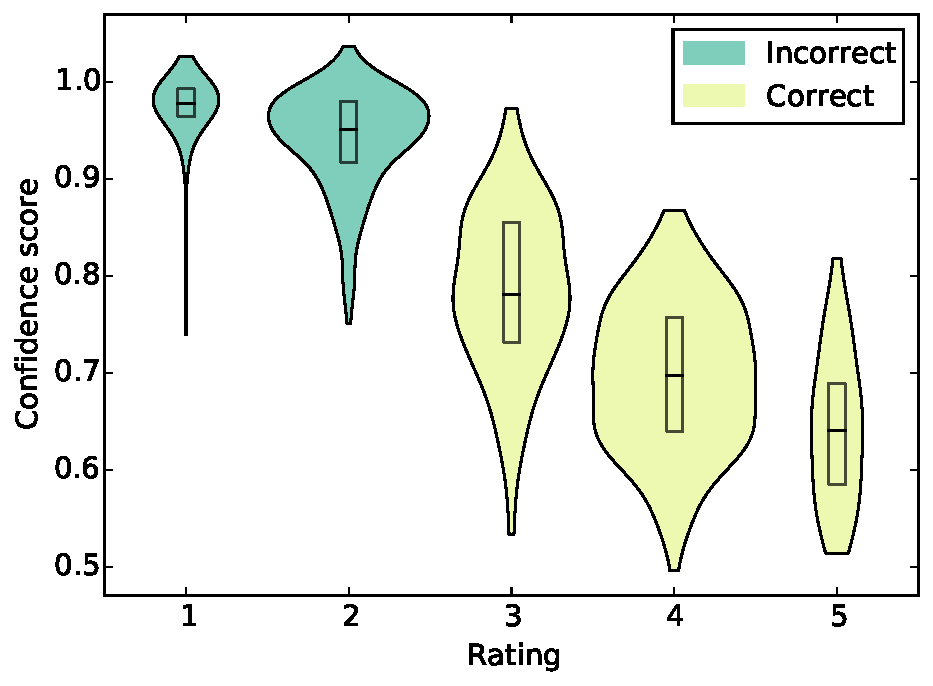
\includegraphics[width=\columnwidth]{violin.pdf}
  \caption{Violin plot (box plot with rotated kernel density estimates) showing the distribution of confidence scores for each rating in our qualitative evaluation.
A smaller confidence score indicates a more successful alignment.
The area of each violin corresponds to the number of pairs which had a given rating.
Box plots in each violin show the median and upper and lower quartiles.}
  \label{fig:violin}
\end{figure}

Figure \ref{fig:violin} shows the distributions of confidence scores for pairs assigned each of the five ratings.
Apart from encountering some incorrect pairs (rated 1), we also found that various transcription issues prevented successful alignments.
A common issue for those pairs rated 2 was that the wrong section of the MIDI transcription was  matched to the audio, often due to different instrumentation, keys, or versions (e.g.\ the audio was a remix).
Any pairs rated 3 either had multiple missing instruments, many musical embellishments, or mismatched tempi.
In addition, the overlap between the confidence scores for pairs rated 4 and 5 indicates that our confidence score is largely invariant to minor transcription issues.
The most common transcription issue for pairs rated 4 was a single missing instrument or minor embellishments, most often on the vocal track.

Overall, our ``gold standard'' alignment system was able to successfully align most correctly-matched pairs and produced a reliable confidence score.
Considering pairs rated 3-5 as ``correct'' matches, the resulting confidence scores achieve an area under the ROC curve of 0.981 (95\% confidence interval [.973, .989], calculated by 1000-sample bootstrap), indicating a high quality measure.
Unfortunately, there were a few pairs rated 1 or 2 that still had small normalized DTW scores suggesting a successful alignment; without these outliers, we could use a wider range of thresholds to obtain high-confidence alignments.
The most important remaining flaw is the relative insensitivity to missing instruments and embellishments.

In summary, large-scale optimization over synthetic data has delivered a DTW-based system which is simple to implement and achieves accurate and reliable results for both alignment and matching.
A high-level discussion of this paper, with more figures and an implementation of our ``gold standard'' system, is available online,\footnote{\href{http://bit.ly/alignment-overview}{\texttt{http://bit.ly/alignment-overview}}} as is the code used in these experiments.\footnote{\href{https://github.com/craffel/alignment-search}{\texttt{https://github.com/craffel/alignment-search}}} 
We thank Hilary Mogul for preliminary work and Dawen Liang for helpful discussion.

\bibliographystyle{IEEEbib}
\bibliography{refs}

\end{document}
